%%%%%%%%%%%%%%%%%%%%%%%%%%%%%%%%%%%%%%%%%
% Programming/Coding Assignment
% LaTeX Template
%
% This template has been downloaded from:
% http://www.latextemplates.com
%
% Original author:
% Ted Pavlic (http://www.tedpavlic.com)
%
% Note:
% The \lipsum[#] commands throughout this template generate dummy text
% to fill the template out. These commands should all be removed when 
% writing assignment content.
%
% This template uses a Perl script as an example snippet of code, most other
% languages are also usable. Configure them in the "CODE INCLUSION 
% CONFIGURATION" section.
%
%Assignment 2
%Author Zetan
%%%%%%%%%%%%%%%%%%%%%%%%%%%%%%%%%%%%%%%%%

%----------------------------------------------------------------------------------------
%	PACKAGES AND OTHER DOCUMENT CONFIGURATIONS
%----------------------------------------------------------------------------------------

\documentclass{article}

\usepackage{fancyhdr} % Required for custom headers
\usepackage{lastpage} % Required to determine the last page for the footer
\usepackage{extramarks} % Required for headers and footers
\usepackage[usenames,dvipsnames]{color} % Required for custom colors
\usepackage{graphicx} % Required to insert images
\usepackage{listings} % Required for insertion of code
\usepackage{courier} % Required for the courier font
\usepackage{multirow}
\usepackage{listings,multicol}

\usepackage{url}

% Margins
\topmargin=-0.45in
\evensidemargin=0in
\oddsidemargin=0in
\textwidth=6.5in
\textheight=9.0in
\headsep=0.25in

\linespread{1.1} % Line spacing

% Set up the header and footer
\pagestyle{fancy}
\lhead{\hmwkAuthorName} % Top left header
\chead{\hmwkClass\ (\hmwkClassInstructor\ \hmwkClassTime): \hmwkTitle} % Top center head
\rhead{\firstxmark} % Top right header
\lfoot{\lastxmark} % Bottom left footer
\cfoot{} % Bottom center footer
\rfoot{Page\ \thepage\ of\ \protect\pageref{LastPage}} % Bottom right footer
\renewcommand\headrulewidth{0.4pt} % Size of the header rule
\renewcommand\footrulewidth{0.4pt} % Size of the footer rule

\setlength\parindent{0pt} % Removes all indentation from paragraphs

%----------------------------------------------------------------------------------------
%	CODE INCLUSION CONFIGURATION
%----------------------------------------------------------------------------------------

\definecolor{MyDarkGreen}{rgb}{0.0,0.4,0.0} % This is the color used for comments
\lstloadlanguages{Python} % Load python syntax for listings, for a list of other languagesftp://ftp.tex.ac.uk/tex-archive/macros/latex/contrib/listings/listings.pdf supported see: 
\lstset{
        frame=single, % Single frame around code
        basicstyle=\small\ttfamily, % Use small true type font
        keywordstyle=[1]\color{Blue}\bf, % python functions bold and blue
        keywordstyle=[2]\color{Purple}, % python function arguments purple
        keywordstyle=[3]\color{Blue}\underbar, % Custom functions underlined and blue
        identifierstyle=, % Nothing special about identifiers                                         
        commentstyle=\usefont{T1}{pcr}{m}{sl}\color{MyDarkGreen}\small, % Comments small dark green courier font
        stringstyle=\color{Purple}, % Strings are purple
        showstringspaces=false, % Don't put marks in string spaces
        tabsize=5, % 5 spaces per tab
        breaklines=true,
        %
        % Put standard python functions not included in the default language here
        morekeywords={rand},
        %
        % Put python function parameters here
        morekeywords=[2]{on, off, interp},
        %
        % Put user defined functions here
        morekeywords=[3]{test},
       	%
        morecomment=[l][\color{Blue}]{...}, % Line continuation (...) like blue comment
        numbers=left, % Line numbers on left
        firstnumber=1, % Line numbers start with line 1
        numberstyle=\tiny\color{Blue}, % Line numbers are blue and small
        stepnumber=5 % Line numbers go in steps of 5
}

% Creates a new command to include a pyton script, the first parameter is the filename of the script (without .py), the second parameter is the caption
\newcommand{\pythonscript}[2]{
\begin{itemize}
\item[]\lstinputlisting[language=python,caption=#2,label=#1]{#1.py}
\end{itemize}
}
% Creates a new command to include a shell script, the first parameter is the filename of the script (without .sh), the second parameter is the caption
\newcommand{\shellscript}[2]{
\begin{itemize}
\item[]\lstinputlisting[language=bash,caption=#2,label=#1]{#1.sh}
\end{itemize}
}
% Creates a new command to include a R script, the first parameter is the filename of the script (without .R), the second parameter is the caption
\newcommand{\Rscript}[2]{
\begin{itemize}
\item[]\lstinputlisting[language=R,caption=#2,label=#1]{#1.R}
\end{itemize}
}
%----------------------------------------------------------------------------------------
%	DOCUMENT STRUCTURE COMMANDS
%	Skip this unless you know what you're doing
%----------------------------------------------------------------------------------------

% Header and footer for when a page split occurs within a problem environment
\newcommand{\enterProblemHeader}[1]{
\nobreak\extramarks{#1}{#1 continued on next page\ldots}\nobreak
\nobreak\extramarks{#1 (continued)}{#1 continued on next page\ldots}\nobreak
}

% Header and footer for when a page split occurs between problem environments
\newcommand{\exitProblemHeader}[1]{
\nobreak\extramarks{#1 (continued)}{#1 continued on next page\ldots}\nobreak
\nobreak\extramarks{#1}{}\nobreak
}

\setcounter{secnumdepth}{0} % Removes default section numbers
\newcounter{homeworkProblemCounter} % Creates a counter to keep track of the number of problems

\newcommand{\homeworkProblemName}{}
\newenvironment{homeworkProblem}[1][Problem \arabic{homeworkProblemCounter}]{ % Makes a new environment called homeworkProblem which takes 1 argument (custom name) but the default is "Problem #"
\stepcounter{homeworkProblemCounter} % Increase counter for number of problems
\renewcommand{\homeworkProblemName}{#1} % Assign \homeworkProblemName the name of the problem
\section{\homeworkProblemName} % Make a section in the document with the custom problem count
\enterProblemHeader{\homeworkProblemName} % Header and footer within the environment
}{
\exitProblemHeader{\homeworkProblemName} % Header and footer after the environment
}

\newcommand{\problemAnswer}[1]{ % Defines the problem answer command with the content as the only argument
\noindent\framebox[\columnwidth][c]{\begin{minipage}{0.98\columnwidth}#1\end{minipage}} % Makes the box around the problem answer and puts the content inside
}

\newcommand{\homeworkSectionName}{}
\newenvironment{homeworkSection}[1]{ % New environment for sections within homework problems, takes 1 argument - the name of the section
\renewcommand{\homeworkSectionName}{#1} % Assign \homeworkSectionName to the name of the section from the environment argument
\subsection{\homeworkSectionName} % Make a subsection with the custom name of the subsection
\enterProblemHeader{\homeworkProblemName\ [\homeworkSectionName]} % Header and footer within the environment
}{
\enterProblemHeader{\homeworkProblemName} % Header and footer after the environment
}

%----------------------------------------------------------------------------------------
%	NAME AND CLASS SECTION
%----------------------------------------------------------------------------------------

\newcommand{\hmwkTitle}{Assignment\ \#5} % Assignment title
\newcommand{\hmwkDueDate}{Thursday,\ March\ 3,\ 2016} % Due date
\newcommand{\hmwkClass}{Web Science\ cs532} % Course/class
\newcommand{\hmwkClassTime}{4:20pm} % Class/lecture time
\newcommand{\hmwkClassInstructor}{Dr.Michael.L.Nelson} % Teacher/lecturer
\newcommand{\hmwkAuthorName}{Zetan Li} % Your name

%----------------------------------------------------------------------------------------
%	TITLE PAGE
%----------------------------------------------------------------------------------------

\title{
\vspace{2in}
\textmd{\textbf{\hmwkClass:\ \hmwkTitle}}\\
\normalsize\vspace{0.1in}\small{Due\ on\ \hmwkDueDate}\\
\vspace{0.1in}\large{\textit{\hmwkClassInstructor\ \hmwkClassTime}}
\vspace{3in}
}

\author{\textbf{\hmwkAuthorName}}
\date{} % Insert date here if you want it to appear below your name

%----------------------------------------------------------------------------------------

\begin{document}

\maketitle

%----------------------------------------------------------------------------------------
%	TABLE OF CONTENTS
%----------------------------------------------------------------------------------------

%\setcounter{tocdepth}{1} % Uncomment this line if you don't want subsections listed in the ToC

\newpage
\tableofcontents
\newpage

%----------------------------------------------------------------------------------------
%	PROBLEM 1
%----------------------------------------------------------------------------------------

% To have just one problem per page, simply put a \clearpage after each problem

\begin{homeworkProblem}
We know the result of the Karate Club (Zachary, 1977) split.
Prove or disprove that the result of split could have been predicted
by the weighted graph of social interactions.  How well does the
mathematical model represent reality?\\
\\
Generously document your answer with all supporting equations, code,
graphs, arguments, etc.\\
\\
Useful sources include:\\
\\
* Original paper\\
\\
\url{http://aris.ss.uci.edu/~lin/76.pdf}\\
\\
* Slides\\
\\
\url{http://www-personal.umich.edu/~ladamic/courses/networks/si614w06/ppt/lecture18.ppt}\\
\\
\url{http://clair.si.umich.edu/si767/papers/Week03/Community/CommunityDetection.pptx}\\
\\
* Code and data\\
\\
\url{http://networkx.github.io/documentation/latest/examples/graph/karate_club.html}\\
\\
\url{http://nbviewer.ipython.org/url/courses.cit.cornell.edu/info6010/resources/11notes.ipynb}
\\
\url{http://stackoverflow.com/questions/9471906/what-are-the-differences-between-community-detection-algorithms-in-igraph/9478989#9478989}\\
\\
\url{http://stackoverflow.com/questions/5822265/are-there-implementations-of-algorithms-for-community-detection-in-graphs}\\
\\
\url{http://konect.uni-koblenz.de/networks/ucidata-zachary}\\
\\
\url{http://vlado.fmf.uni-lj.si/pub/networks/data/ucinet/ucidata.htm#zachary}\\
\\
\url{https://snap.stanford.edu/snappy/doc/reference/CommunityGirvanNewman.html}\\
\\
\url{http://igraph.org/python/doc/igraph-pysrc.html#Graph.community_edge_betweenness}\\

\centerline{SOLUTION}
First, we have to get the raw data of karate club network from the official data site of igraph called Nexus.\url{http://nexus.igraph.org/api/dataset_info?id=1&format=html}\\
Then plot the original network out.\\

\begin{figure}
\centering
\caption{original karate club network}
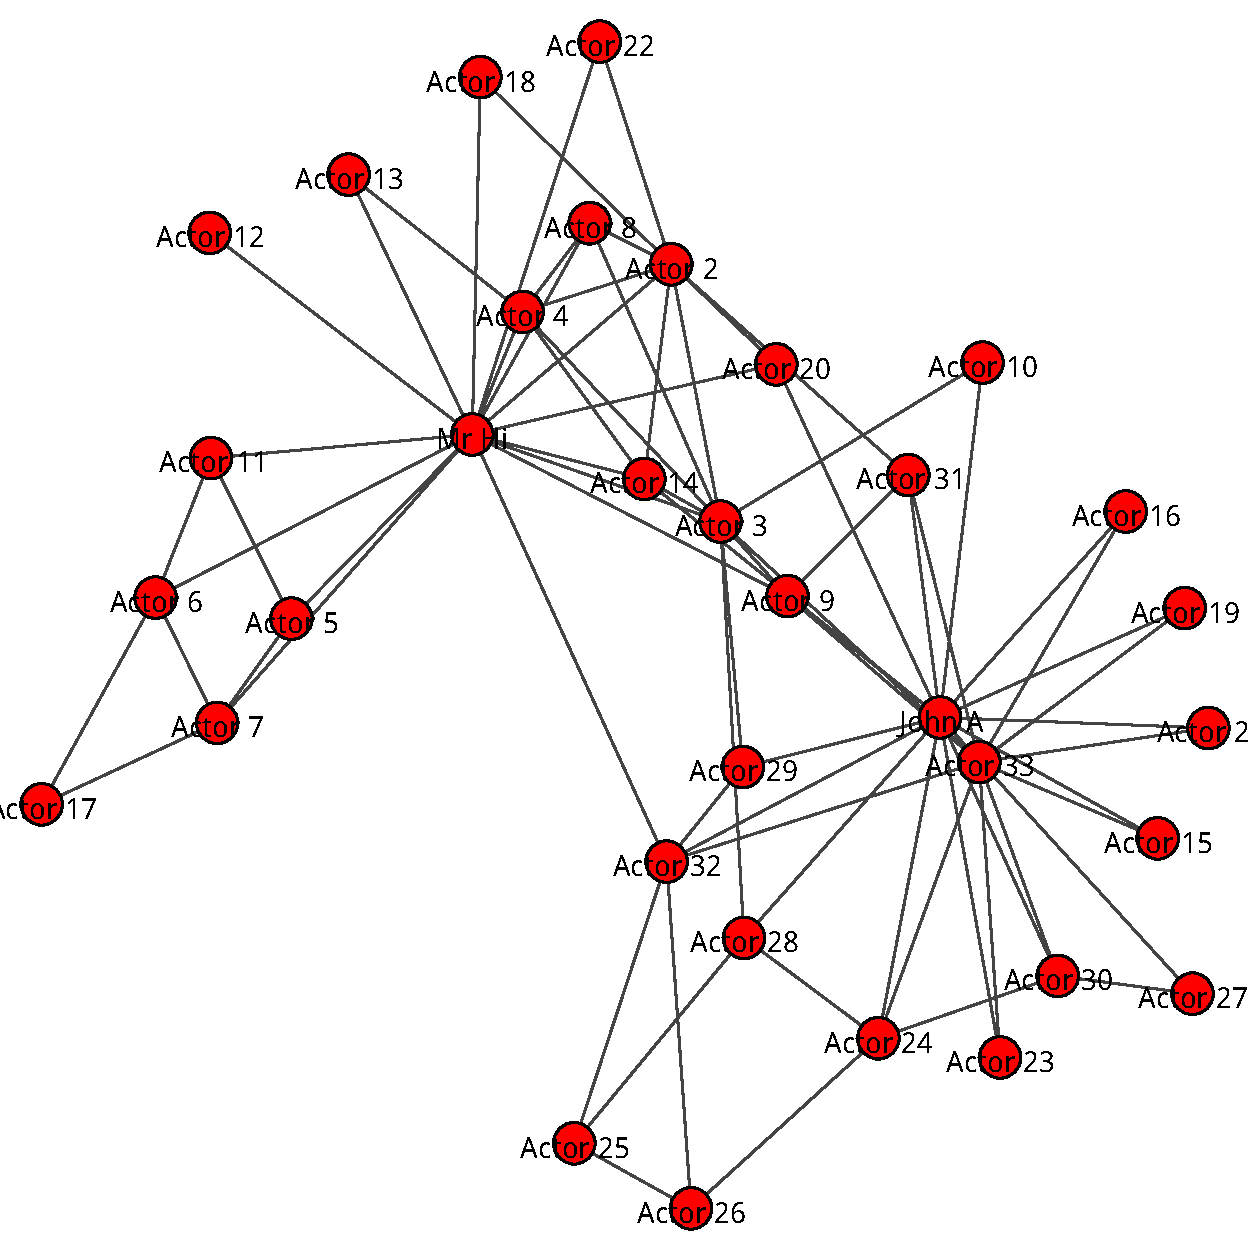
\includegraphics[scale=.5]{p1_org}
\end{figure}
Then in the original data file (karate.graphml), we find there is a data field called ``Faction''. This indicates the original subgroup architecture. So we set the node to different colour according to the  faction number they have. We will use this to compare with the prediction made by algorithm.\\
\begin{figure}
\centering
\caption{original karate club network subgroups}
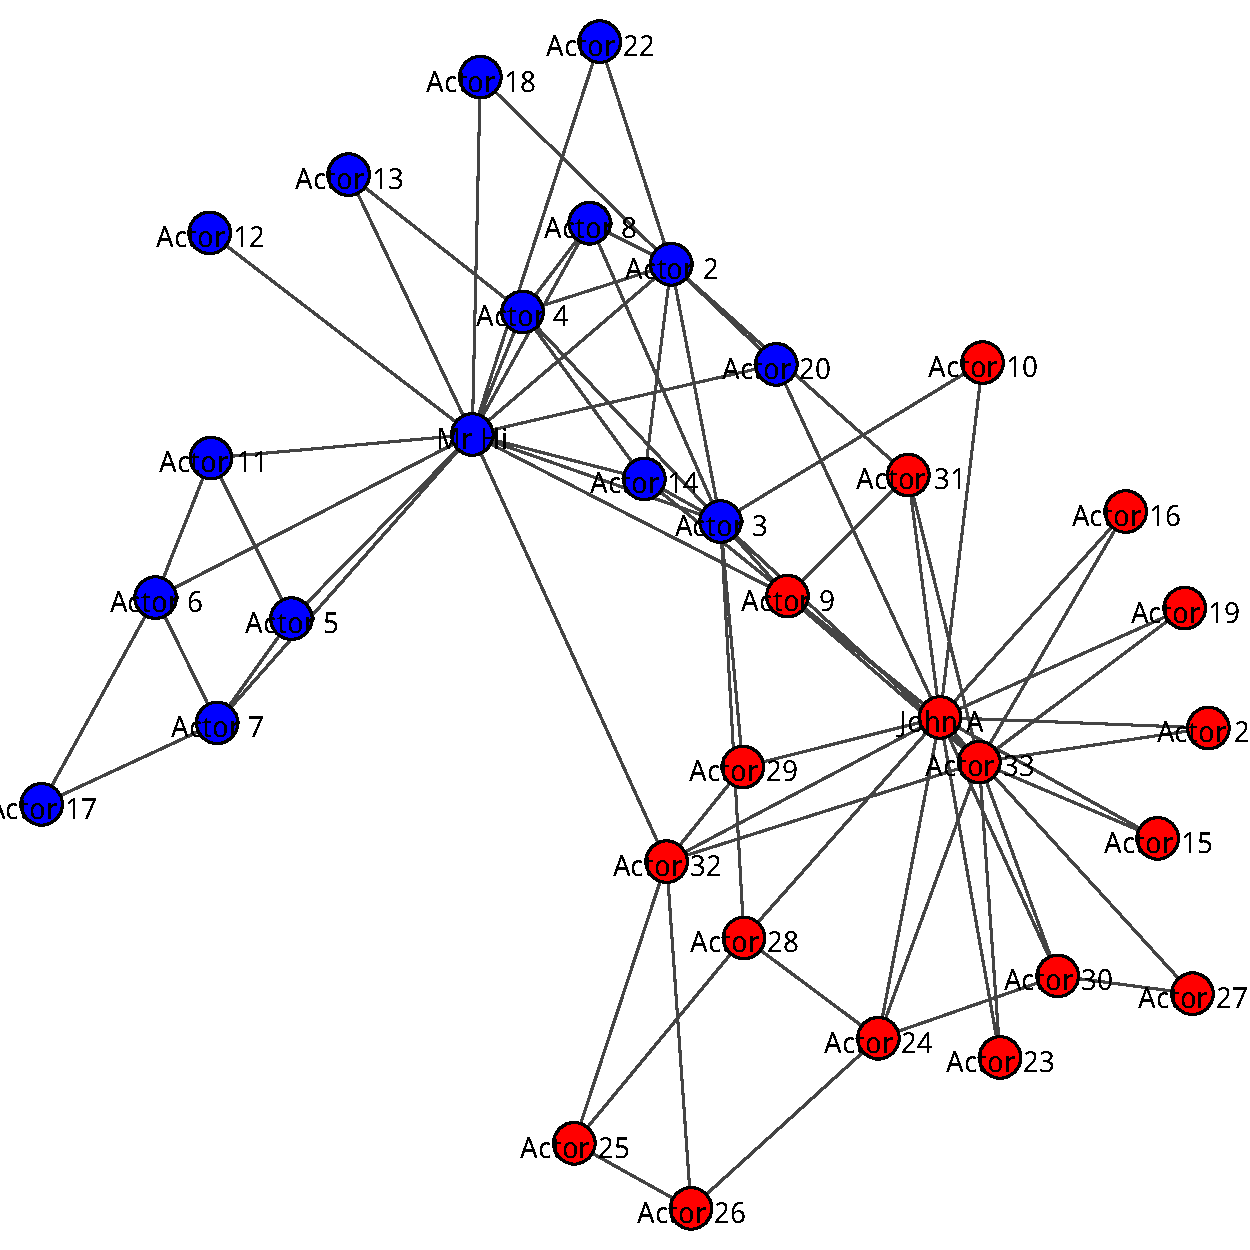
\includegraphics[scale=.5]{p1_org_split}
\end{figure}

Now comes the betweenness algorithm, the igraph library has this feature in the graph module.
Above is the graph output split by the betweenness algorithm.

\begin{figure}
\centering
\caption{Predicted karate club network }
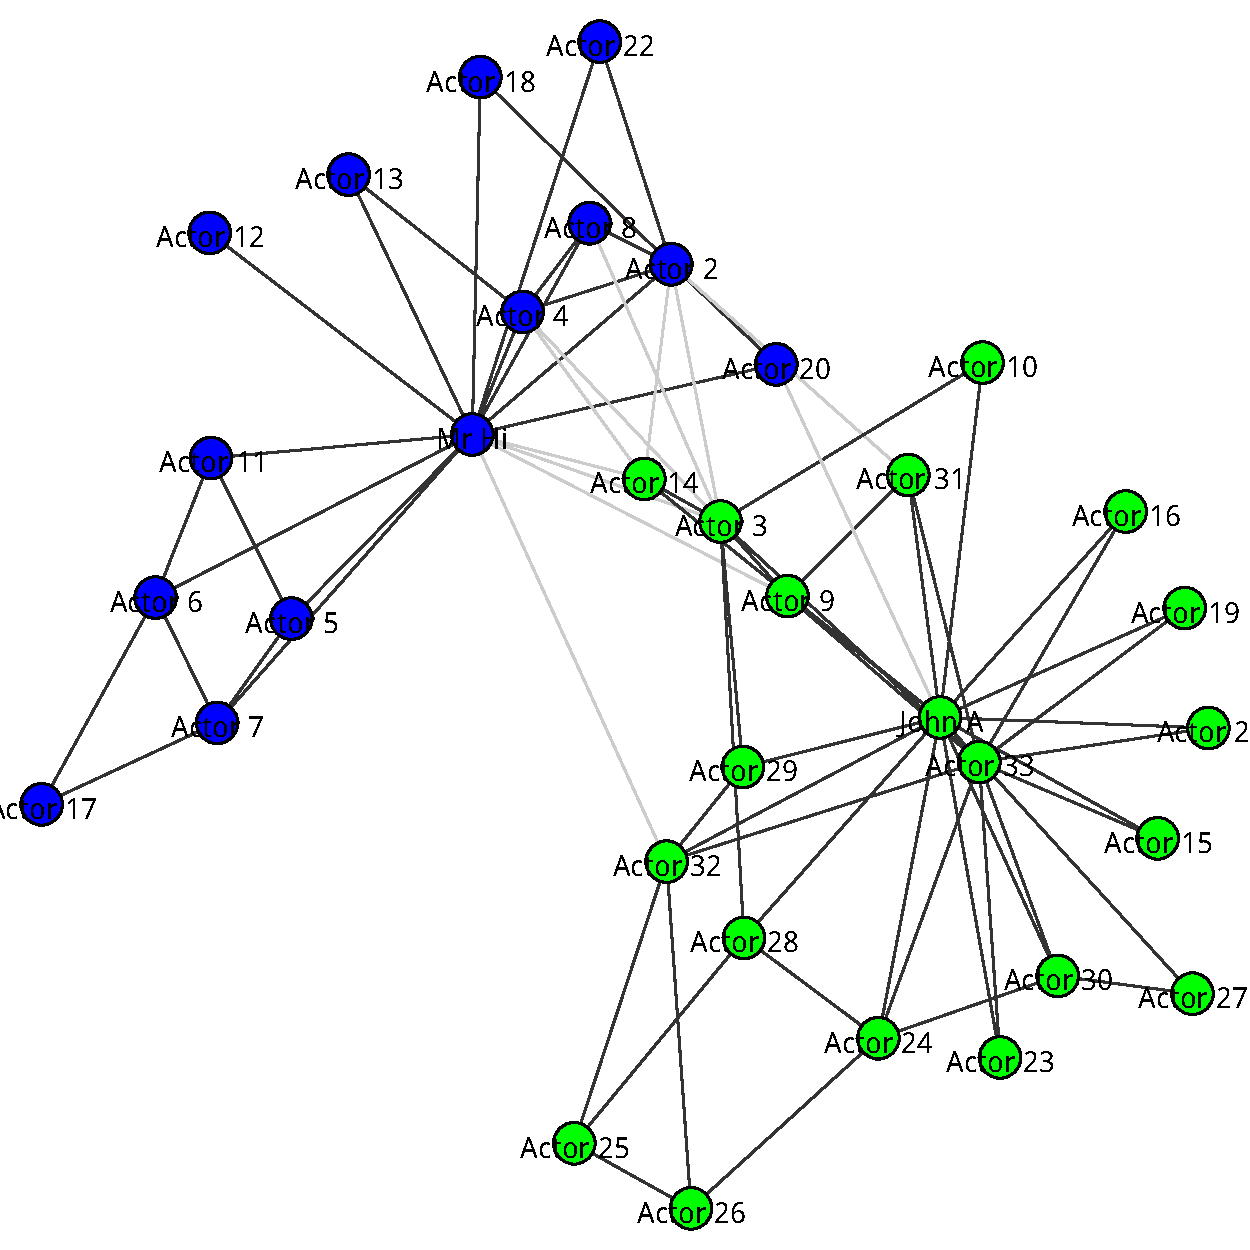
\includegraphics[scale=.5]{p1_cut}
\end{figure}

\pythonscript{p1}{python code to plot original graph and predicted graph}
From the predicted graph, we can see that there are only two node in wrong group: Actor14 and Actor3.\\
So the total accuracy is 94.11\%
\end{homeworkProblem}
\pagebreak
%----------------------------------------------------------------------------------------
%	PROBLEM 2
%----------------------------------------------------------------------------------------
\begin{homeworkProblem}
We know the group split in two different groups.  Suppose the
disagreements in the group were more nuanced -- what would the clubs
look like if they split into groups of 3, 4, and 5?\\
\centerline{SOLUTION}
The betweennes algorithm in igraph have an option called `clusters', which enable us to specify the certain number of subgroups we want in splitting. 
\pythonscript{p2}{python code to plot predicted graph in 3\,4\,5 subgroups}
\pagebreak
\begin{figure}
\centering
\caption{Predicted karate club network in 3 subgroups}
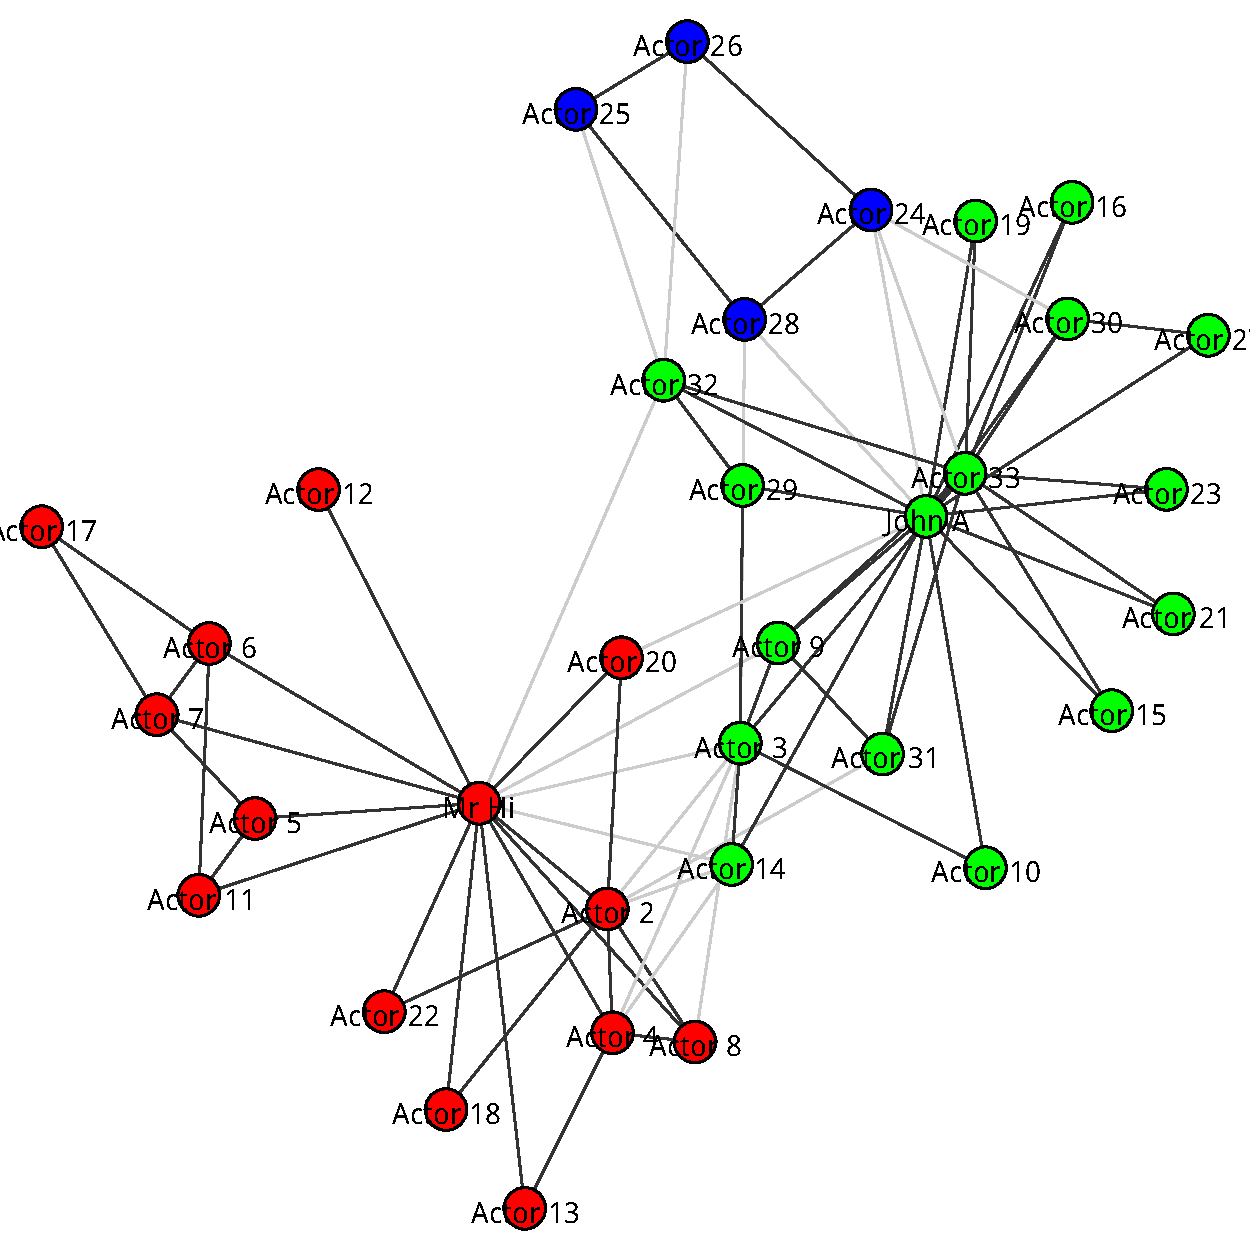
\includegraphics[scale=.5]{p2_cluster3}
\caption{Predicted karate club network in 4 subgroups}
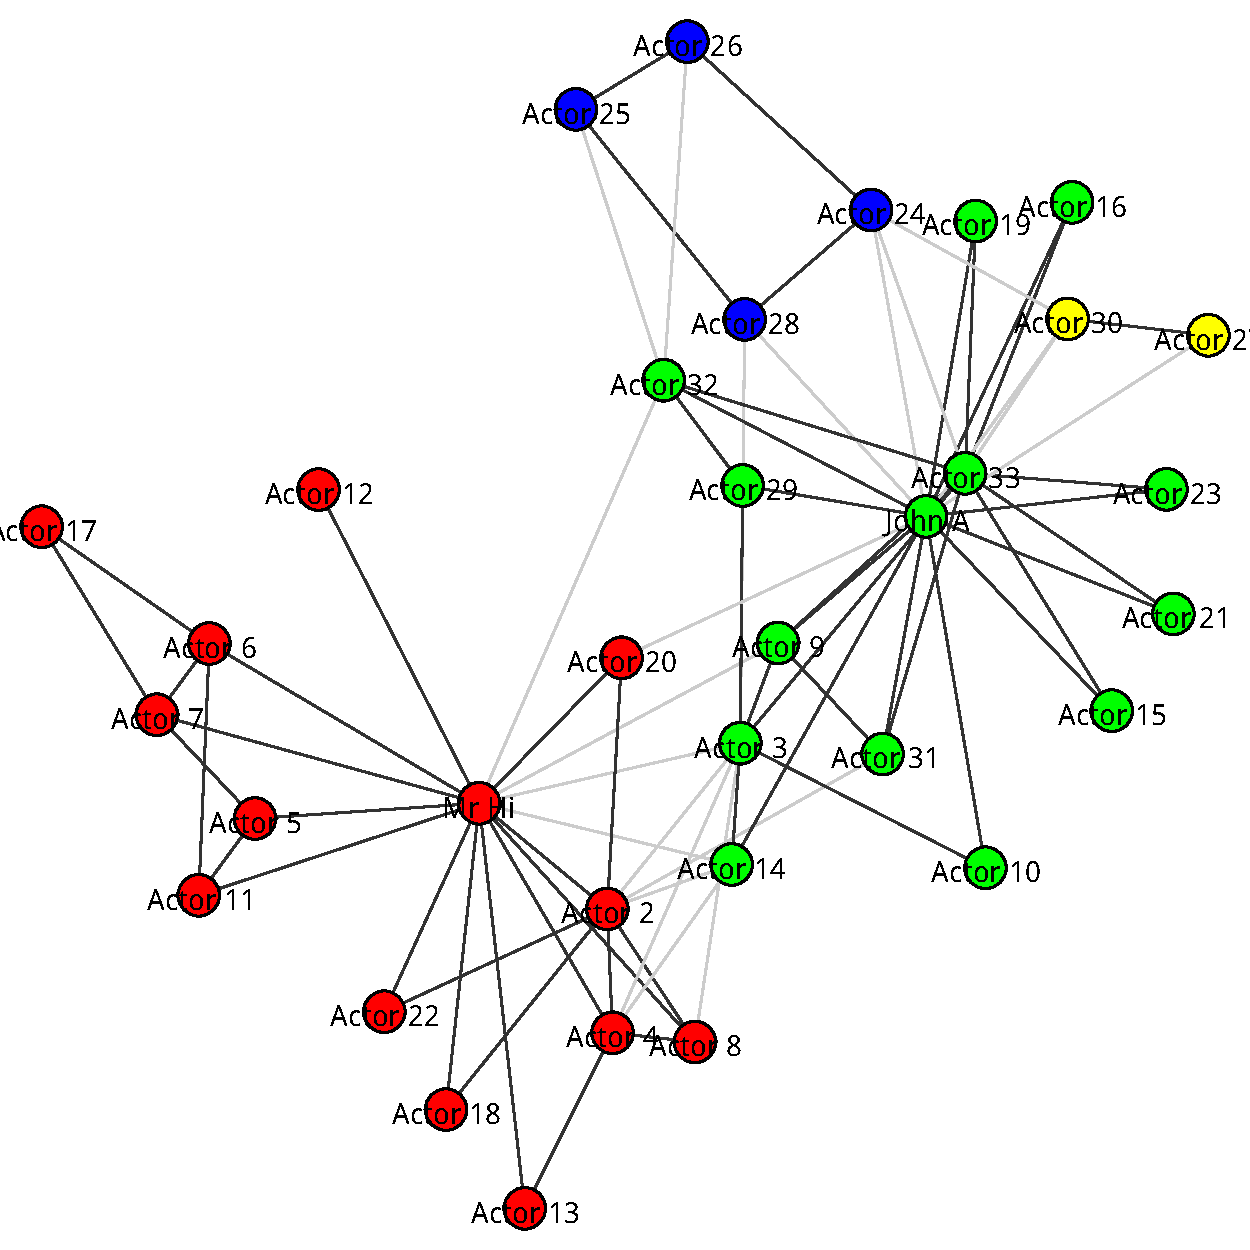
\includegraphics[scale=.5]{p2_cluster4}
\end{figure}
\begin{figure}
\centering
\caption{Predicted karate club network in 5 subgroups}
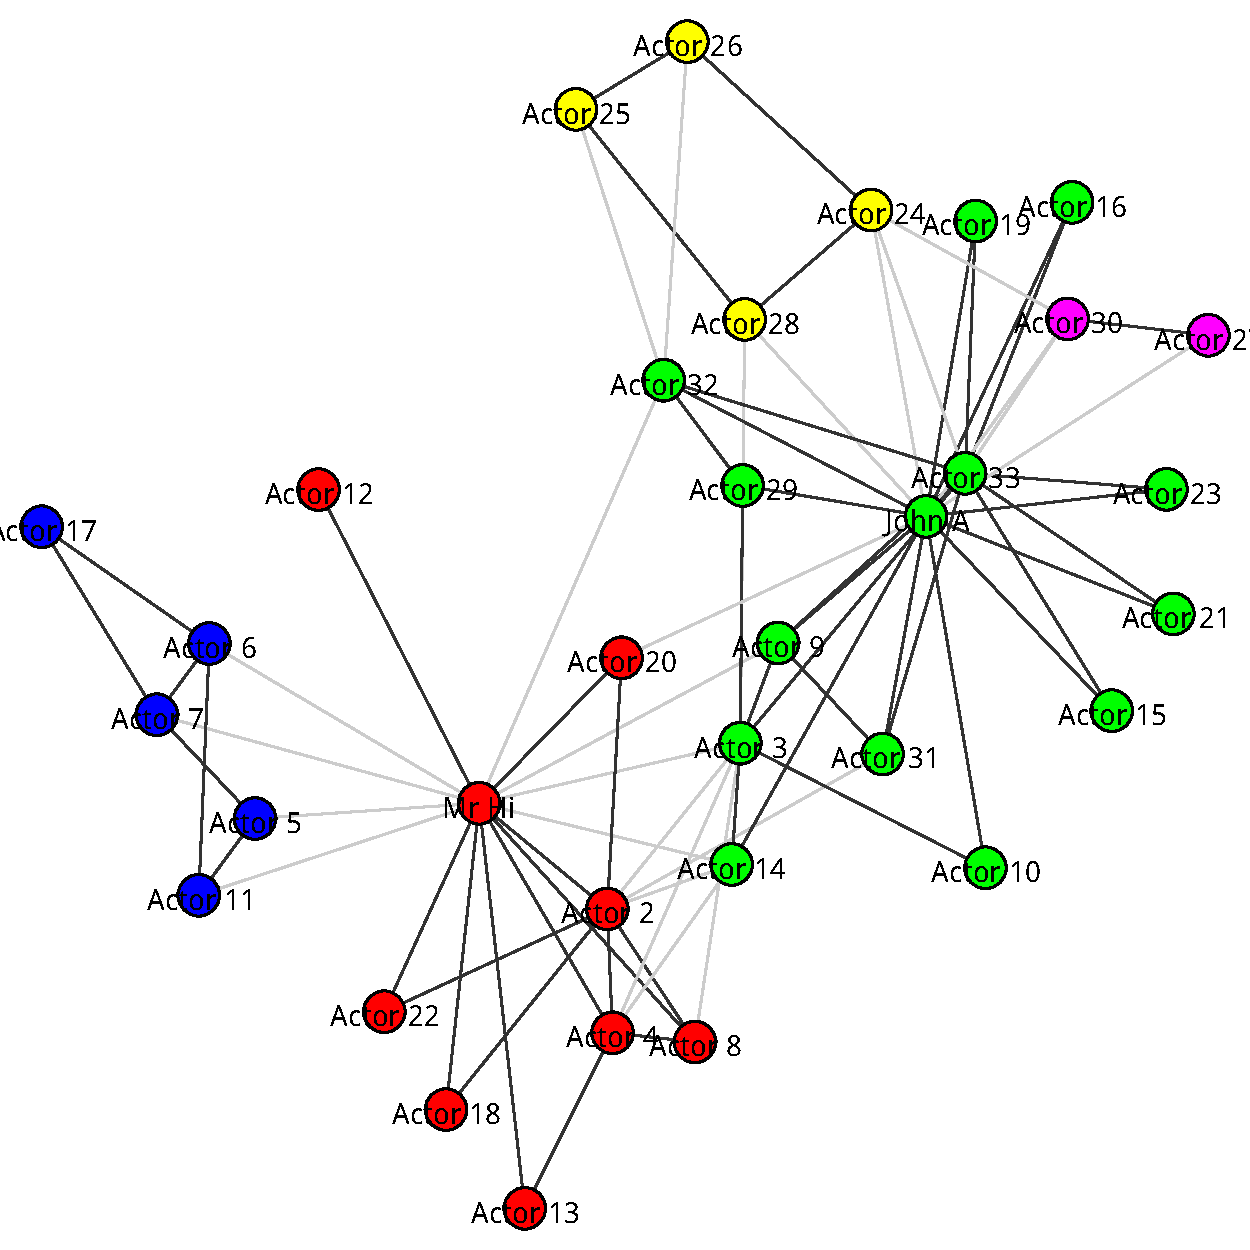
\includegraphics[scale=.5]{p2_cluster5}
\end{figure}
\end{homeworkProblem}
%\bibliographystyle{plain}
%\bibliography{ref}
\end{document}